\documentclass{sig-alternate}
\usepackage[english]{babel}
\usepackage{url}
\usepackage{booktabs}
\setlength{\heavyrulewidth}{1.2pt}
\setlength{\lightrulewidth}{0.7pt}
\usepackage{enumitem}%Na zoznamy
\usepackage{hyperref}%Na cross referencie
\usepackage[labelfont=bf]{subfig}%pre podobrazky a nastavenie tucneho fontu pre podobrazky
\usepackage[labelfont=bf]{caption}%Tucny font pre nazov obrazka

\usepackage{algpseudocode}%Rozlozenie (layout) pre algoritmus
\usepackage{amsmath}%Vzorce
\usepackage[linesnumbered,ruled,vlined]{algorithm2e}%Algoritmus
\SetCommentSty{mycommfont}%Vzhlad komentarov v algoritme

\usepackage{fancyhdr}%Hlavicka
\renewcommand{\headrulewidth}{0pt}%Odstranenie podciarknutia z hlavicky
\pagestyle{fancy}%Style hlavicky
\lhead{EdRecSys: Educational Recommender Systems}%Lava strana hlavicky
\rhead{UMAP’17, July 9-12, 2017, Bratislava, Slovakia}%Prava strana klavicky
\pagenumbering{arabic}%Cislovanie stranok
\setcounter{page}{153}%Zacatie cislovania stranok od 153

\usepackage{graphicx}%Obrazky
\usepackage{float}%Plavajuce objekty.(obrazky a tabulky)

\usepackage[square,numbers]{natbib}%Bibliografia
\bibliographystyle{abbrv}%Style bibliografie
\setlength{\bibsep}{0.0pt}%Odstranenie medzier medzi odsekami bibliografie
\renewcommand*{\bibfont}{\scriptsize}%Zmensenie velkosti textu bibliografie

\makeatletter
\def\@copyrightspace{\relax}%Odstranenie ACM ISBN a DOI z prvej strany 
\makeatother

\begin{document}
\title{RUTICO:Recommending Successful Learning Paths under Time Constraints}
\numberofauthors{3}
\author{
\alignauthor
Amir Hossein Nabizadeh* \\
       \affaddr{LIAAD,INESC TEC,Porto}\\
       \affaddr{Faculdade de Ciências}\\
       \affaddr{Universidade do Porto}\\
       \affaddr{Porto,Portugal}\\
       \email{amirhossein@dcc.fc.up.pt}
\alignauthor
Alípio Mário Jorge\\
       \affaddr{LIAAD,INESC TEC,Porto}\\
       \affaddr{Faculdade de Ciências}\\
       \affaddr{Universidade do Porto}\\
       \affaddr{Porto,Portugal}\\
       \email{amjorge@fc.up.pt}
\alignauthor
José Paulo Leal\\
       \affaddr{LIAAD,INESC TEC,Porto}\\
       \affaddr{Faculdade de Ciências}\\
       \affaddr{Universidade do Porto}\\
       \affaddr{Porto,Portugal}\\
       \email{zp@dcc.fc.up.pt}
}
\maketitle

\begin{abstract}
    Nowadays using E-learning platforms such as Intelligent Tutoring Systems (ITS) that support users to learn subjects are quite common. Despite the availability and the advantages of these systems, they ignore the learners’ time limitation for learning a subject. In this paper we propose RUTICO, that recommends successful learning paths with respect to a learner’s knowledge background and under a time constraint. RUTICO, which is an example of Long Term goal Recommender Systems (LTRS), after locating a learner in the course graph, it utilizes a Depth-first search (DFS) algorithm to find all possible paths for a learner given a time restriction. RUTICO also estimates learning time and score for the paths and finally, it recommends a path with the maximum score that satisfies the learner time restriction. In order to evaluate the ability of RUTICO in estimating time and score for paths, we used the Mean Absolute Error and Error. Our results show that we are able to generate a learning path that maximizes a learner’s score under a time restriction.
\end{abstract}

\begin{flushleft}
\ccsdesc{Information systems~\textbf{Recommender systems}}
\ccsdesc{Applied computing
~\textbf{E-learning}}
\ccsdesc{Mathematics of computing~\textbf{Graph algorithms}}
\printccsdesc
\end{flushleft}

\begin{keywords}
 Long Term Goal Oriented Recommenders (LTRS), E-learning, Recommendation System (RS), Depth-first search (DFS).
\end{keywords}
\section{INTRODUCTION}
\label{sec:introduction}
\noindent E-learning systems aim to deliver educational resources to users. These systems have been able to progressively remove the barriers of space and time by delivering educational resources anytime and anywhere. E-learning systems have several advantages compared to traditional learning methods, such as reducing cost, availability, flexibility (give users the freedom to learn at their own convenience), etc \cite{dargham2012learning}. In these systems, if a user plans to learn a course, he/she requires to spend a specified amount of time, which is often fixed and given by the system. The problem is if a learner’s available time is less than the required time by the system, the learner might not be able to learn the materials properly. Therefore the learner fails to complete a learning process (i.e. dropout problem \cite{crawford2013community}) and subsequently his/her obtained learning score from the course could not be good. Long Term goal Recommender Systems (LTRS) \cite{nabizadeh2015long} can be used as a possible solution to address the learners’ time constraint. The LTRS, beside satisfying current needs of learners (what they need to learn immediately) and engaging them more with the system by personalizing the learning materials , guide them toward a predefined goal by generating a set of relevant strategic recommendations. In our study, the predefined goal is obtaining the maximum possible learning score in a limited time. The LTRS method that we present (RUTICO) uses a graph traversal algorithm to generate personalized learning paths from a course graph. In a course graph, nodes represent the learning objects (LO) and directed edges indicate the prerequisite relations among the LO. To traverse the course graph, Depth First Search (DFS) algorithm
\cite{tarjan1972depth} is used in order to generate all paths from an initial point, which is defined by a learner. RUTICO also estimates the learning time and score for each generated path using the transaction data and finally, it recommends a path that satisfies the learner’s time restriction while maximizing his/her score. Our proposal has three main contributions:

\begin{enumerate}[noitemsep,label=(\arabic*)]
\item RUTICO provides personalized support for learners. This assists both the learners and teachers to be more productive.
\item RUTICO uses the learners’ transaction data to estimate learning score and time for the target learner. Researchers often estimate a learning time and score for a path which is a fixed value for all learners, while our estimation methods estimate personalized learning time and score for each learner.
\item Our method considers the learners’ time limitation and personalizes the learning process under the learner’s time restriction.
\end{enumerate}

The remainder of this paper is structured as follows: section \ref{sec:relatedwork} introduces related work and section \ref{sec:problemdefinition} clarifies our problem in detail. Our method is described in section \ref{sec:ruticomethod} which utilizes the DFS algorithm as the basis. The data description and evaluation methodology are mentioned in section \ref{sec:evaluationanddiscussion}. Finally, in section \ref{sec:conclusion}, we present our conclusion.
\newpage
\section{RELATED WORK}
\label{sec:relatedwork}
\noindent Over the last decade, E-learning systems have been researched extensively in the various approaches. Several E-learning systems use a Course Generation approach (CG) where the entire learning path is generated and recommended to a learner in a single recommendation. If a learner is not able to follow the path, the recommender generates another one \cite{belacel2014binary,durand2013graph,ullrich2010complex}. This method has been frequently used by researchers along with various techniques and algorithms. Vassileva and Deters \cite{vassileva1998dynamic} introduced a method that works based on previous knowledge of a learner and his/her goal, and can be updated dynamically with respect to the learner progress. Their proposal, given a concept (goal), utilizes an AO* algorithm \cite{bundy1986catalogue} to search for paths in an AND/OR concept graph \cite{de1990and} that connect the concepts known by the learner with the goal concept. Finally, the recommendation of their method is a sequence of teaching materials (each concept has a set of teaching material) for a target learner.

CourseNavigator, that is proposed by Li et al., relies on a graph search algorithm. It generates all paths given a set of learners’ inputs. The inputs are constraints (e.g., maximum number of courses to take per semester, courses to avoid), educational goal (e.g., graduation semester, a set of desired courses), student’s enrollment status (e.g. starting point), and their preferred ranking for the output paths (e.g., shortest, most reliable, etc.). Their method then is able to generate three types of paths: (a) deadline-driven paths (paths that end by a given semester), (b) goal-driven paths (meet student goal by a given semester) and (c) ranked paths (based on the studentfis ordering preferences) \cite{nabizadeh2015long}. In their method, the recommended path is a sequence of semesters that in each semester a learner needs to take a definite number of courses regardless of time that each course may take in that semester. Adorni and Koceva presented a method to generate learning path by means of Educational Concept Maps (ECM) \cite{adorni2015designing}. Their personalization process starts with a self-verification of knowledge by a learner which cause pruning the known topics from the ECM map. The output of pruning process will be checked, and finally, by specifying the initial and target point (topic) by the learner, the paths will be generated using ENCODE that performs an algorithm to linearize the map \cite{adorni2016educational}.

In CG, there are studies such as \cite{durand2011learning} and \cite{farrell2004dynamic} that consider the learners’ time restriction. In their methods, although these two studies use different methods to recommend paths, the time of each LO is static (assigned by a course designer) and represented in the metadata of the LO, and time for a path is estimated by accumulating the learning time of LO in that path. For example, a model that is proposed by Farrell et al., receives a learner’s inputs (topic keywords, time restriction, and search scope that specifies how much a learner intends to focus on a topic) to generate personalized learning paths under a time constraint. In their method, dynamic assembly of LO is based on the relative match of the LO metadata (LOM) to the learner’s needs, preferences, and constraints \cite{farrell2004dynamic}.

Alternatively, the Course Sequence (CS) method, unlike the CG approach, recommends LO one by one as the learner progresses \cite{li2012self}. Different solutions have been proposed, using a Neural Network \cite{idris2009adaptive}, Evolutionary Algorithms (EAs) \cite{li2016coursenavigator} and other algorithms and approaches. Karampiperis and Sampson \cite{li2012self} presented an Adaptive Educational Hypermedia System (AEHS) \cite{brusilovsky1996methods}. In their work, goals are divided into three main categories: (1) cognitive capability and skills, (2) practical capabilities and skills, and (3) additional transferable skills. Their method, generates all possible learning paths that obtain the goal, and it then selects a path adaptively based on a decision model \cite{karampiperis2004adaptive}. This decision model matches the features of LO with the characteristics and preferences of a target learner. Govindarajan et al. introduced a method using Parallel Particle Swarm Optimization (PPSO) to predict a dynamic learning path for learners. Their method clusters learners into four groups based on their proficiency level. The proficiency includes both measuring the achievement of a target outcome, and the competence and metacompetence changes during the learning process for each defined learning outcome. Second, it predicts the dynamic path based on the clustered information \cite{govindarajan2016dynamic}.

\section{PROBLEM DEFINITION}
\label{sec:problemdefinition}
\noindent In this paper, our main goal is to recommend a sequence of LO that maximizes a learner’s score under a given time restriction (our proposal is a CG method). These sequences (paths) need to be generated from a course graph. Each LO of this course graph has two main attributes: time and score (Figure \ref{fig:f1}). These two attributes refer to the learning time and score of learners who already selected the LO. In Figure \ref{fig:f1}, we show an example of our problem where we intend to find a path that gives the best learning score for a learner who already knows LO 3, while satisfying his/her $T_u$ (the learner’s time restriction).

\begin{figure}[H]
    \centering
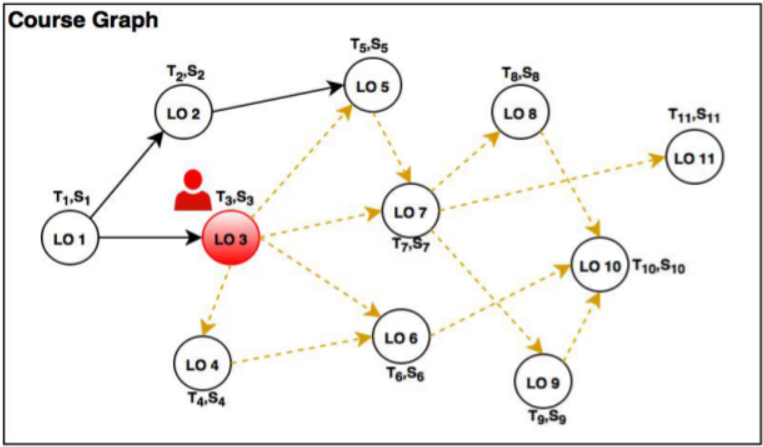
\includegraphics[width=0.8\linewidth]{images/figure1.png}
    \caption{\textbf{Course graph. Each LO has two attributes: time
and score (T,S). The dash links show the potential paths for
the learner who is located in LO 3.}}
    \label{fig:f1}
\end{figure}

In order to tackle the problem, we divide our problem into three sub-problems that are mentioned below. In our problem definition, \textit{D} is the usage data, \textit{G} is the course graph, $T_u$ representing time restriction of a learner u, $T_p$ shows the estimated time of path \textit{P, sp} depicts the current position of \textit{u} (e.g. LO3 in Figure \ref{fig:f1}) and finally \textit{u} that represents the target learner ID.

The sub-problems that we need to overcome are:

\begin{enumerate}[noitemsep,label=(\arabic*)]
\item \textbf{Path Generation}: Generating all possible paths \textit{P} for a learner \textit{u} regarding his/her knowledge background \textit{sp} and
his/her time restriction $T_u$.
\item \textbf{Time estimation}: Estimating learning time for a generated path $P\ (T_p)$.
\item \textbf{Score estimation}: Estimating learning score for a path \textit{P} $(S_p)$.
\end{enumerate}

\newpage
Regarding the sub-problems, we can formalize our main problem in the form of equation \ref{eq:1}.

\begin{equation} \label{eq:1}
Max Score (P) where T_p \leq T_u
\end{equation}

\section{RUTICO METHOD}
\label{sec:ruticomethod}
\noindent As mentioned in section \ref{sec:problemdefinition}, RUTICO approach is divided into three main phases which are path generation, time estimation and score estimation. In this section, we describe our method (Algorithm \ref{alg:1}) in detail, explain how we generate paths from the course graph, and what are our methods in order to estimate the learning score and time for the personalized paths.

\subsection{Path generation}
\label{subsec:pathgeneration}
\noindent In RUTICO, by identifying the starting point sp by a target learner \textit{u} (line 2 in Algorithm \ref{alg:1}), the depth-first-search (DFS) which is a well-known algorithm is utilized to generate all possible paths from the course graph \textit{G} that start by \textit{sp}. The DFS is selected since as we exhaustively search the graph and enumerate all possible paths, DFS statistically consumes less memory for its stack in comparison to the queue of Breadth First Search (BFS) algorithm \cite{bundy1984breadth}. Therefore, for scalability reasons (the BFS may need too much memory and impractical to use) the DFS is chosen. The generated paths must satisfy the learner’s time restriction (time estimation in section \ref{subsec:timeestimation}).

\subsection{Time estimation}
\label{subsec:timeestimation}
\noindent To estimate the time for each path, RUTICO estimates the learning time of each LO (a path consists of several LO) for the target learner. For time estimation, we consider four different methods (results are in section \ref{sec:evaluationanddiscussion}). In \textbf{Mean} and \textbf{Median} methods, we calculate the time’s mean and median of other learners that already selected a target LO. Besides the \textbf{Mean} and \textbf{Median} methods, we propose a time estimation method which is called \textbf{User Adjusted.Mean}
(UA.Mean) by using equations \ref{eq:2} and \ref{eq:3} (\textbf{UA.Median} method follows the same instruction as \textbf{UA.Mean} while it uses the median instead of mean). The purpose of introducing the \textbf{UA.Mean} and \textbf{UA.Median} for time estimation is to estimate how fast is a target learner in comparison to the rest of the learners in learning the LO.

In equation \ref{eq:2}, the numerator $(t_{uLOi})$ refers to the learning time of learning object \textit{i} that is already visited by the target learner \textit{u}, and the denominator $(mean(t_{.LOi}))$ indicates the average learning time of other learners on learning object \textit{i}. \textit{n} shows the total number of LO that are visited by \textit{u}.

\begin{equation} \label{eq:2}
R_u = \frac{1}{n} \sum_{i=1}^n \frac{t_{uLOi}}{mean(t_{.LOi})}
\end{equation}

Then, the learning time of $LO_x$ ($LO_x$ is not visited by the target learner) can be calculated by a multiplication between the $R_u$ and the average learning time of other learners that already visited the $LO_x$ (equation \ref{eq:3}). Eventually, learning time of a path will be estimated by summing the learning time of LO in that path.

\begin{equation} \label{eq:3}
t_x = R_u \times mean(t_{.LOx})
\end{equation}

RUTICO keeps generating a path (i.e. adding LO to the end of a path) as long as the estimated time for that path follows the time condition (i.e. $T_P \leq T_u$). If the estimated time of a path reach the time restriction of the learner, RUTICO stops adding LO to that path and starts generating another path.

\subsection{Score estimation}
\label{subsec:scoreestimation}
\noindent To estimate the score, we consider the same instructions (methods) as time estimation while using the score of LO instead of time. Since in our data the learners’ scores for LO are represented in the form of 0 (fail) and 1 (pass), therefore our score estimation infers a learner’s ability to complete a LO. Hence, in score estimation, \textbf{UA.Mean} and \textbf{UA.Median} methods indicate how good is a target learner in completing a LO in comparison to the rest of the learners. Finally, by estimating the score for all paths, our method recommends a path that gives the maximum score (see Algorithm \ref{alg:1}).


\begin{algorithm}
\caption{RUTICO algorithm.}
\label{alg:1}
    \SetKwInOut{Input}{Input}
    \SetKwInOut{Output}{Output}
    \Input{\textit{u,sp,$T_u$,G,D}.}
    \Output{A path that gives the best score while satisfies $T_u$.}
    Recom[] $\leftarrow$ empty;    \Comment{Recom is a list.}\\
    node $\leftarrow$ sp;\\
    P $\leftarrow$ [sp];  \Comment{P is a list.}\\
    i $\leftarrow$ 1;\\
    $T_P \leftarrow T_{sp}$;  \Comment{\textit{T}:time.Calculated using equations \ref{eq:2}\&\ref{eq:3}}\\
    $S_P \leftarrow S_{sp}$;    \Comment{\textit{S}:score.}\\
    \textbf{Algorithm DFS} ($node,G,S_P,T_P,T_u ,P,i,Recom$)
    
    \Begin{
     \eIf{(\textit{edgelist of \textbf{node} = empty})}{ 
         Recom[i] $\leftarrow$ ($P,T_P,S_P$);\\
         i++;\\
         }
     {\ForEach{ (\textit{Newnode in edgelist of node})}
            {\If{($T_P\ + T_{newnode}\ <=\ T_u$)}{
         $T_P + = T_{Newnode}$;\\
         $S_P + = S_{Newnode}$;\\
         \textit{P $\leftarrow$ P + Newnode};\\
         \textbf{DFS} ($Newnode,G,P,T_P,S_P$);
         }
         \Else{Recom[i] $\leftarrow$ ($P,T_P,S_P$);\\
        i++;
        }
        }
     }
    }
    Final Path $\leftarrow$ \textbf{return} \textit{the \textbf{Recom} . \textbf{Recom}  is a set of paths that are listed in descending order by score.}
\end{algorithm}

\section{EVALUATION AND DISCUSSION}
\label{sec:evaluationanddiscussion}
\noindent To evaluate our method we used one dataset that includes two kinds of data, usage data and a course graph. Our data is taken from a web-based learning environment for programming languages named Enki \cite{paiva2016enki}. This data is for the C\# programming language course which was conducted by the Polytechnic Institute of Porto in academic year 2015/2016.

\newpage
\subsection{Enki Dataset}
\label{subsec:enkidataset}
\noindent The Enki usage data consist of 1186 learners’ transactions for 61 learners. This data includes 8 attributes that are listed below.

\begin{itemize}[noitemsep]
\item \textbf{User ID} : 61 unique IDs.
\item \textbf{Resource ID} : 59 different LO that are in the form of URLs.
\item \textbf{Title}: Title of each resource id.
\item \textbf{State}: Indicates the status of each LO for each learner and can have four different values: Available, Unavailable, Seen and Solved. If a LO is accessible to a learner the status value would be Available, and Unavailable otherwise.
\item \textbf{Grade} : 0 and 1. A grade for a LO is 1 only if a learner could solve (i.e. ”Solved” state) the LO and for the rest of the states the grade would be 0.
\item \textbf{Learning time} : Time to learn each LO by the learners per millisecond. Min $\approx$ 0, Max = 490 minutes.
\item \textbf{Type} : Shows the type of each LO. Type Problem indicates the question and Video refers to the expository LO. In our data, we have 36 problems and 23 videos.
\item \textbf{Learning Object ID} : Learning objects’ ID (resource ID).
\end{itemize}

The Enki course graph, designed by a course expert, consists of 59 LO and 83 links. The links indicate the prerequisite relation among the LO.

\subsection{Result and Discussion}
\label{subsec:resultanddiscussion}
\noindent In this section, we describe our experiments. Since we applied the DFS which is an off-the-shelf algorithm to traverse a graph, we do not evaluate the DFS. Here, we assess the ability of four different methods (described in section \ref{sec:ruticomethod}) for estimating the learning time and score of each LO for a target learner. To evaluate the estimation methods, we have used the Mean Absolute Error (MAE) and Error.

To evaluate the performance of our estimation methods, we take a sequence of LO that a learner already visited. We then ignore some of the LO from the sequence and consider them as unobserved LO (Figure \ref{fig:f2}), and attempt to estimate time and score of unobserved LO. For ignoring the LO we use a window. A window is composed of unobserved LO, and its size ranges from 1 to 10. Every time we ignore a number of LO (it depends on the size of the window) for a learner and estimates their time and score. We then calculate the MAE between the estimated time and score of unobserved LO and their actual values (Figures \ref{fig:f3} and \ref{fig:f4}). The purpose of using different window size is to check which method consistently performs better than the rest of approaches.

\begin{figure}[H]
    \centering
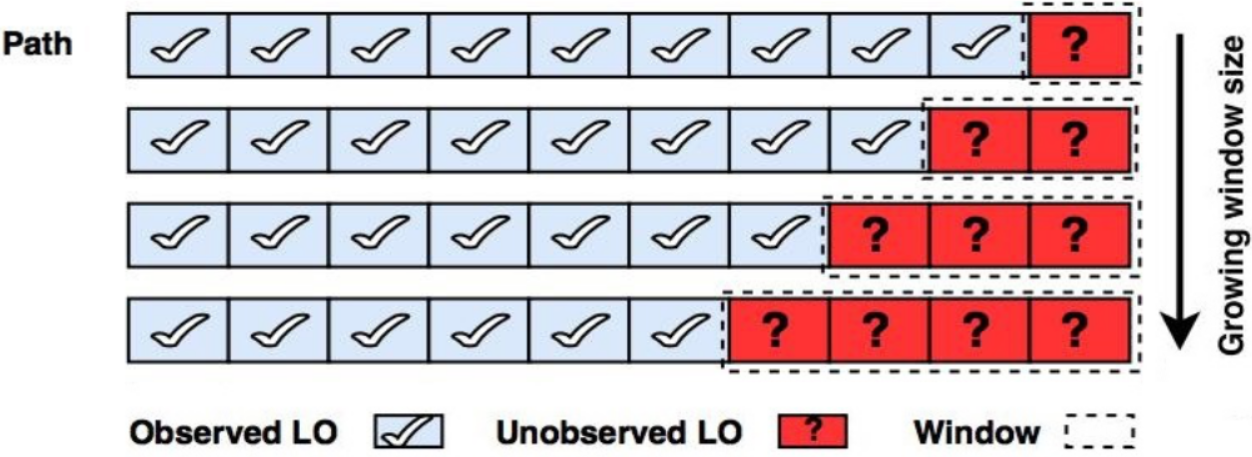
\includegraphics[width=0.8\linewidth]{images/figure2.png}
\caption{\textbf{Evaluation method. For a path, the time and score
of observed LOs are used to estimate the unobserved ones.}}
    \label{fig:f2}
\end{figure}

\begin{figure}[H]
\centering
\subfloat[\textbf{Learning Time estimation. Timescale is in minutes.}\label{fig:f3a}]{
  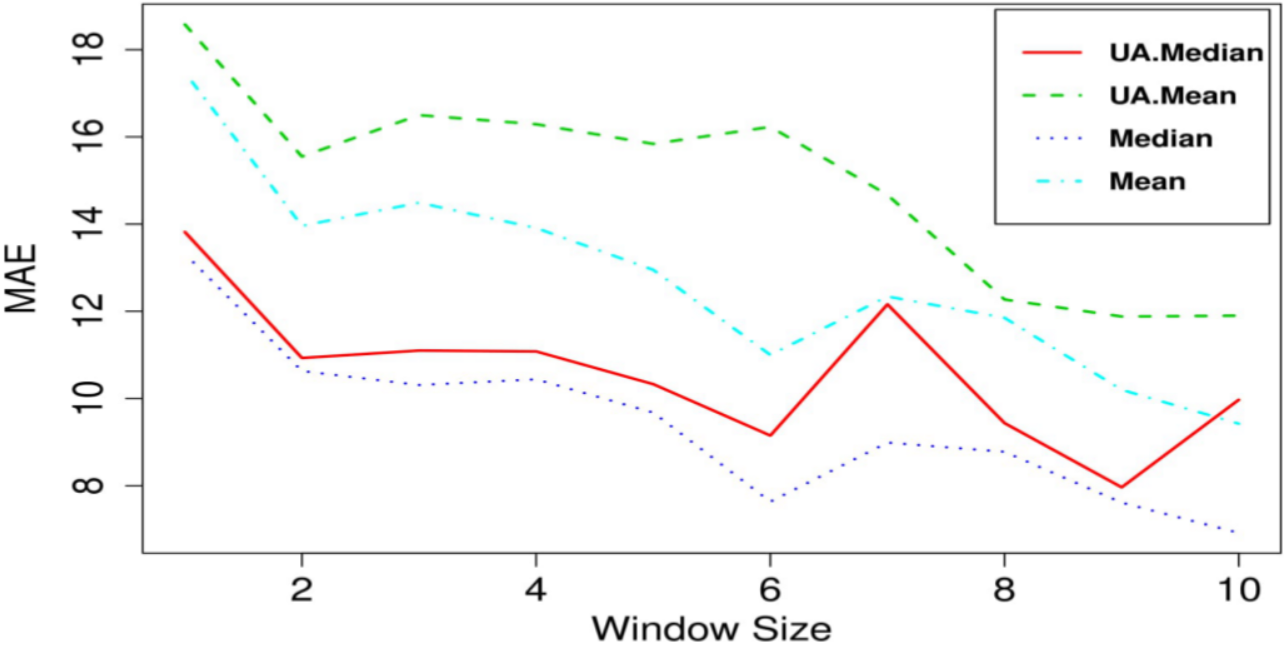
\includegraphics[width=0.8\linewidth]{images/figure3a.png}
  }\par        
\subfloat[\textbf{Learning Score estimation.
}\label{fig:f3b}]{
  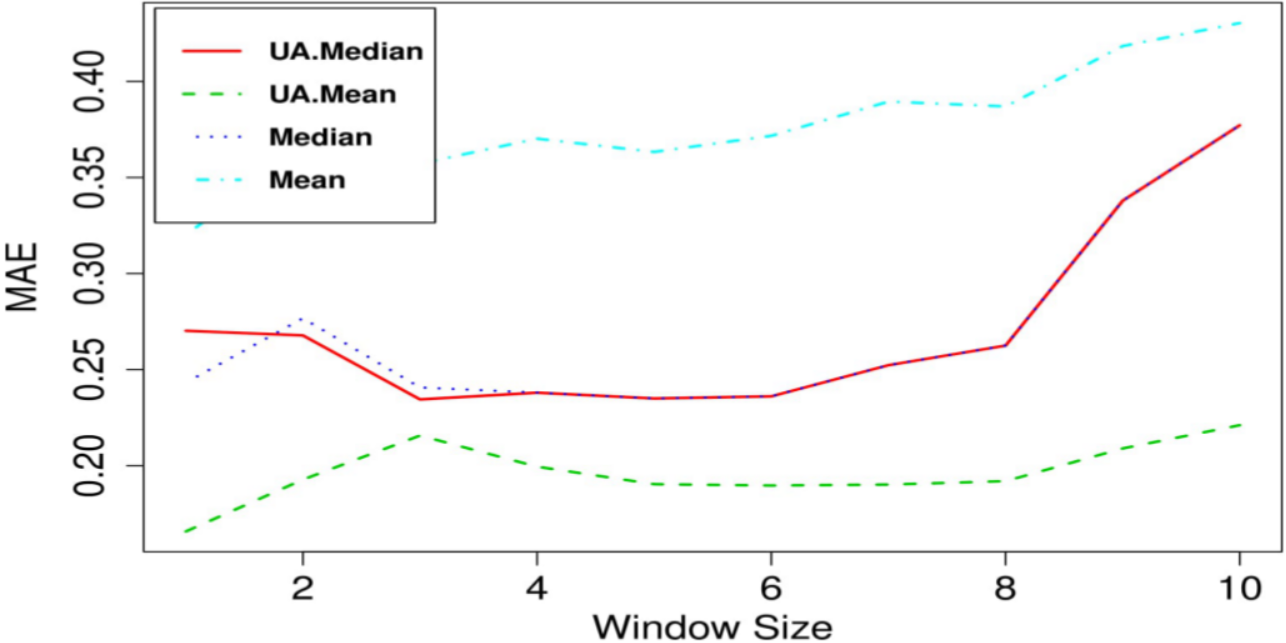
\includegraphics[width=0.8\linewidth]{images/figure3b.png}
  }
\caption{\textbf{Mean Absolute Error for time and score estimation.}}
\label{fig:f3}
\end{figure}

\subsubsection{Evaluating estimation methods}
\label{subsubsec:evaluatingestimationmethods}
\noindent In this section, we intend to evaluate the ability of the methods to correctly estimate the learning time and score of LO for a target learner. In Figure \ref{fig:f3}, we consider both types of LO together (Problems and Videos as described in section \ref{subsec:enkidataset}). According to the results in Figure \ref{fig:f3}, \textbf{UA.Mean} performs better than the other methods in score estimation, while \textbf{Median} approach outperforms other methods for time estimation. In addition, Figure \ref{fig:f3} shows that the error increases by decreasing the size of the window. It happens since learners were devoted more to the course at the beginning. Therefore, the data is less noisy which results in less error in time estimation. During the time that the learners lose their learning motivation, the data gets more noise and the error increases. In the case of score, unlike the time, error increases by increasing the size of the window since the score is independent from learners’ devotion to the course.

In order to check how different types of LO influence the results, we estimate the time and score for expository (Video) and evaluative (Problem) LO separately. Since the expository LO has no grade (only Problems have grades), we only estimate the learning time for different types of LO (results are in Figure \ref{fig:f4}).

According to the results in Figure \ref{fig:f4}, the \textbf{Median} could have a better performance than the other approaches in estimating time for the LO. By comparing the results in Figure \ref{fig:f3a} with the results in Figure \ref{fig:f4}, we conclude that considering different types of LO separately will reduce the error, especially for expository LO (Videos).

Regarding the results that are represented in Figures \ref{fig:f3} and \ref{fig:f4}, the \textbf{UA.Mean} outperforms the other three approaches in score estimation, while in time estimation the results are competitive and the best result is obtained by using the \textbf{Median} method.

\newpage
\begin{figure}[H]
\centering
\subfloat[\textbf{Expository type (Video). Timescale is in minutes.}\label{fig:f4a}]{
  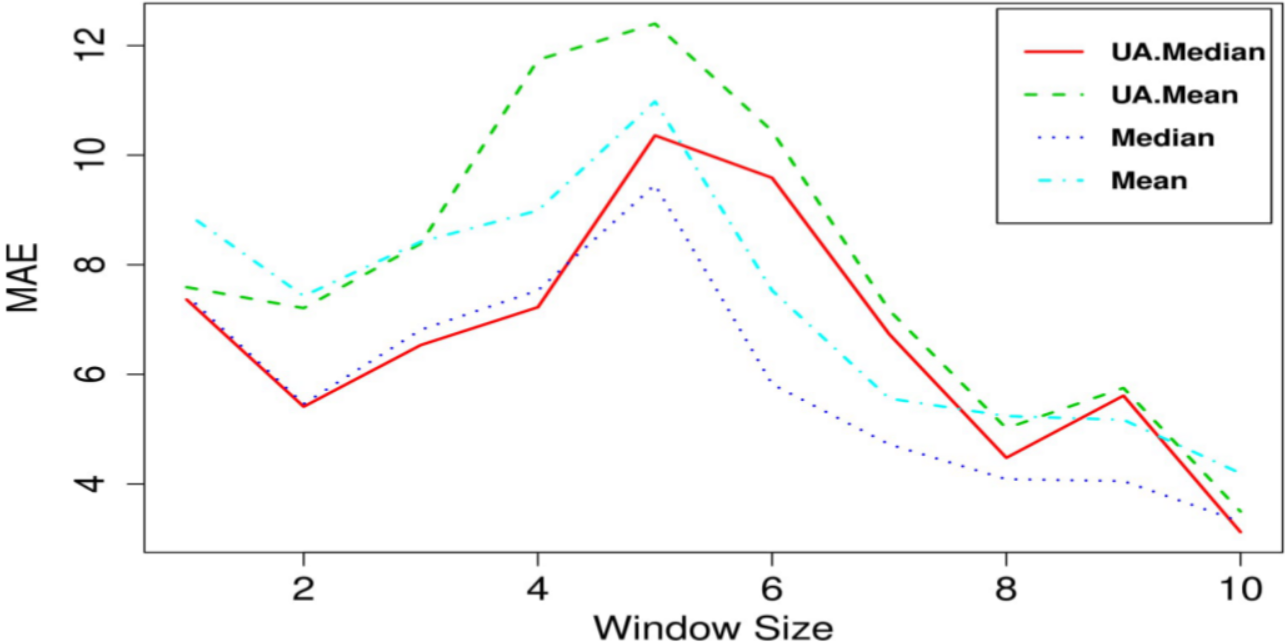
\includegraphics[width=0.8\linewidth]{images/figure4a.png}
  }\par        
\subfloat[\textbf{Evaluative type (Problem). Timescale is in minutes.}\label{fig:f4b}]{
  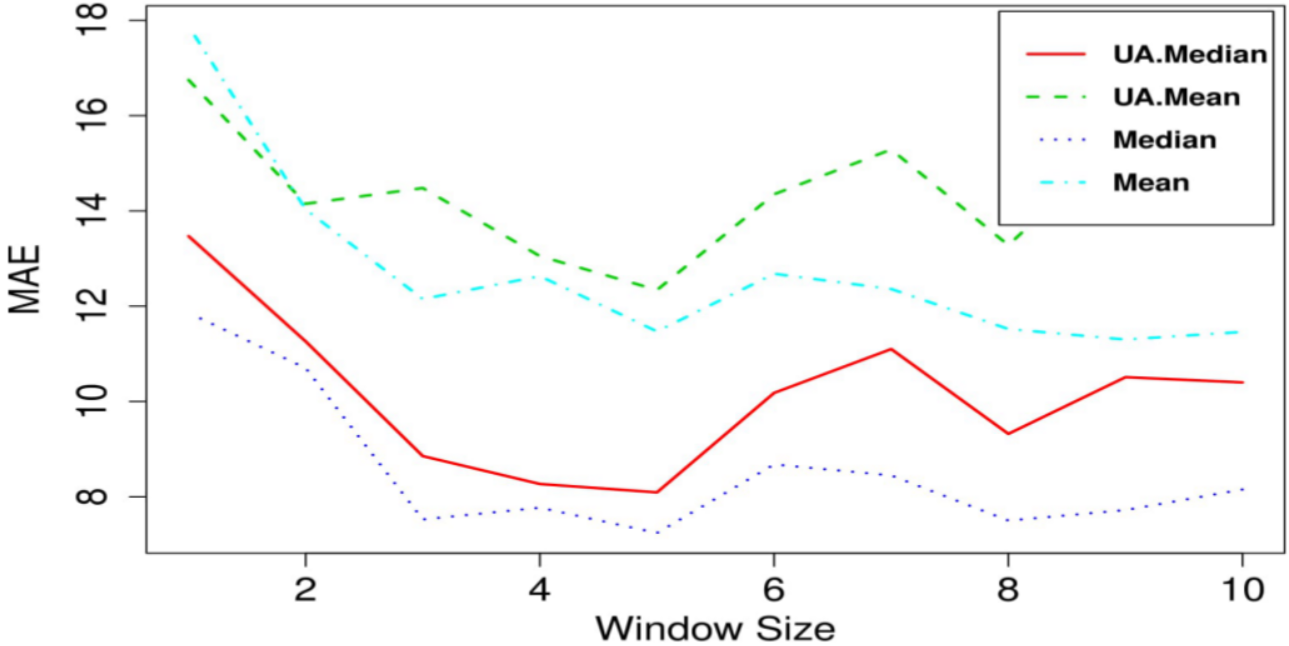
\includegraphics[width=0.8\linewidth]{images/figure4b.png}
  }
\caption{\textbf{Mean Absolute Error for different LO.}}
\label{fig:f4}
\end{figure}

\subsubsection{Evaluating overestimation and underestimation of the selected approaches}
\label{subsec:evaluatingoverestimation}
\noindent By identifying the appropriate methods for estimating time and score, we evaluated the selected approaches by using estimation error. The error results are shown in the form of probability density (Figures \ref{fig:f5} and \ref{fig:f6}) to show the percentage of overestimation (estimated values > real values) and underestimation (estimated values < real values) of the selected methods. In learning time, underestimation indicates higher risk than overestimation since a learner might not complete a generated path in the estimated time. Unlike time, score overestimation signifies higher risk because a learner may not obtain the estimated score from a path.

In Figures \ref{fig:f5} and \ref{fig:f6}, the orange highlighted part (negative error) indicates the underestimation and the blue part (positive error) shows the overestimation. By comparing the results in Figure \ref{fig:f5a} with the results in Figure \ref{fig:f6}, we see that considering different types of LO separately reduces the error while increases the type of underestimation error. Since the learning time of LO varies from $\approx$zero to $\approx$500 minutes, $\approx$10 (for videos) and $\approx$20 minutes (for problems) can be considered as minor errors.

\subsection{RUTICO example}
\label{subsec:ruticoexample}
\noindent Figure \ref{fig:f7} shows an example of our proposal for generating a path for a target learner. It generates learning paths that start by the
starting point of the learner (LO 13) under a given time restriction. Regarding the evaluation results, \textbf{Median} and \textbf{UA.Mean} are the selected methods to estimate the learning time (we estimate time for different type of LO separately) and score of LO respectively. In our example, the RUTICO uses the time and score of LO 1, 3, 4, 5 and 9 (i.e. observed LO) of the learner along with the time and

\begin{figure}[H]
\centering
\subfloat[\textbf{Time estimation using Median approach. Timescale
is in minutes.}\label{fig:f5a}]{
  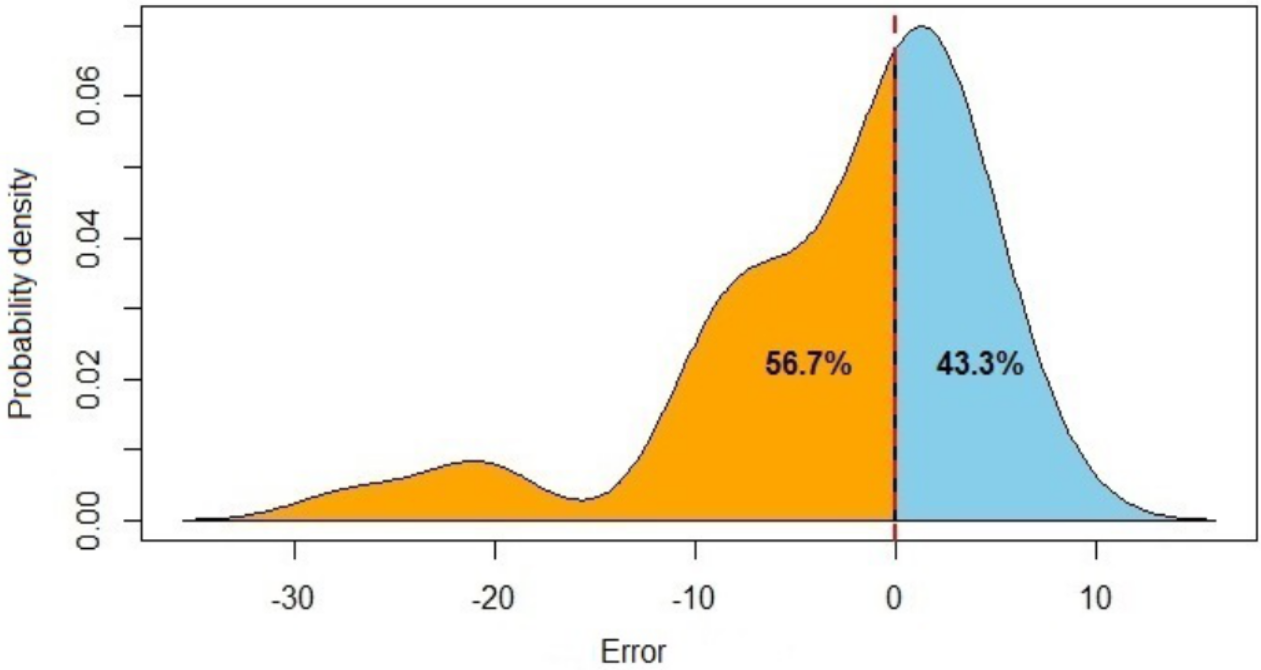
\includegraphics[width=0.8\linewidth]{images/figure5a.png}
  }\par        
\subfloat[\textbf{Score estimation using UA.Mean approach.}\label{fig:f5b}]{
  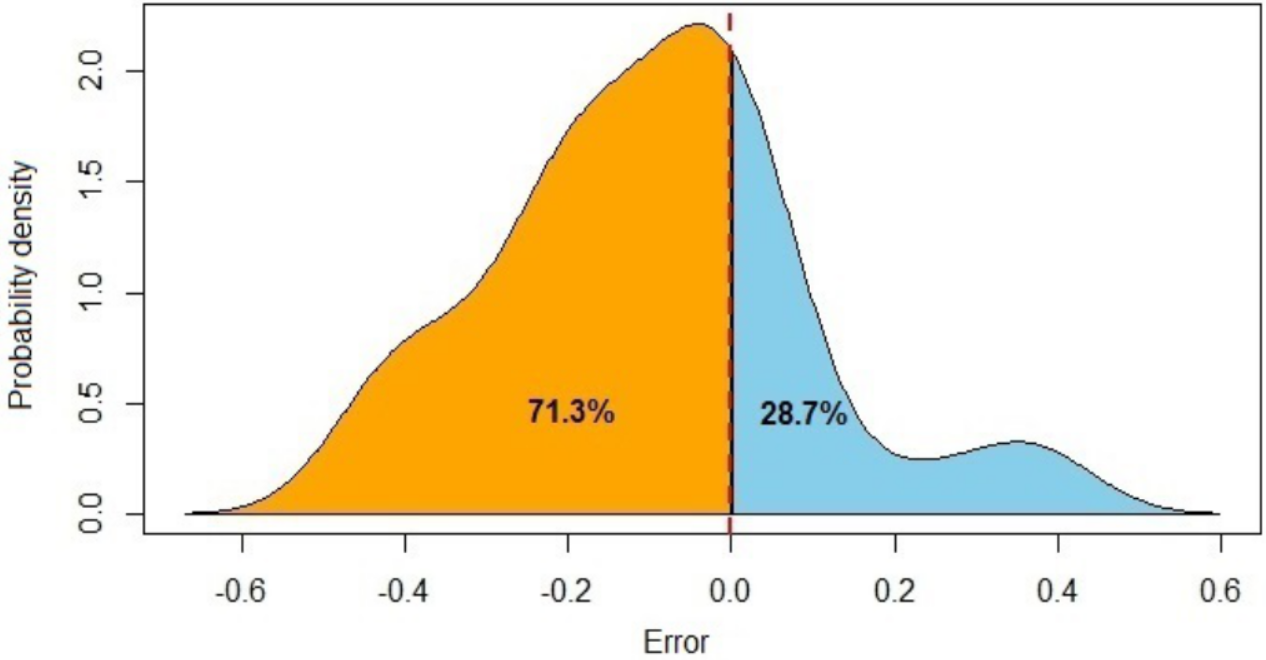
\includegraphics[width=0.8\linewidth]{images/figure5b.png}
  }
\caption{\textbf{Probability density of Error for time and score es-
timation.}}
\label{fig:f5}
\end{figure}

score of other learners that they already visited the LO that are in the generated paths to estimate the time and score of the paths for the target learner. Finally, RUTICO recommends a path with maximum score to the learner.

\section{CONCLUSION}
\label{sec:conclusion}
\noindent In this paper, we propose our method RUTICO to recommend a sequence of Learning Objects (LO) that maximizes a learner’s score under his/her time restriction. Our approach works by exploiting two kinds of data, i.e., usage data and a course graph. The method uses the Depth First Search (DFS) algorithm to generate all paths for a learner from his/her starting point in the course graph, estimates score and time for all generated paths and finally recommends a path with the maximum score that satisfies the learner time limitation. We evaluate the result of the four different methods that are for estimating time and score in order to select the best one for estimating the time and score of LO.

In the future, we aim to tackle the learner cold-start problem, extend our method to an adaptable one (i.e. can be updated regarding the learners progress), automatically identifying the starting point of a learner in a course graph, deal with uncertainty for estimating time and score, and evaluate our method in a live environment to assess the quality of the recommendations.

\section*{ACKNOWLEDGMENTS}
\label{sec:acknowledgments}
This work is financed by the ERDF - European Regional Development Fund through the Operational Programme for Competitiveness and Internationalisation - COMPETE 2020 Programme
\newpage

\begin{figure}[t]
\centering
\begin{minipage}{.5\textwidth}[t]%Tu som pouzil minipage aby som dal obrazok 7 napravo od tychto dvoch obrazkov.
  \centering
  \subfloat[\textbf{Expository type (Video).}\label{fig:f6a}]{
  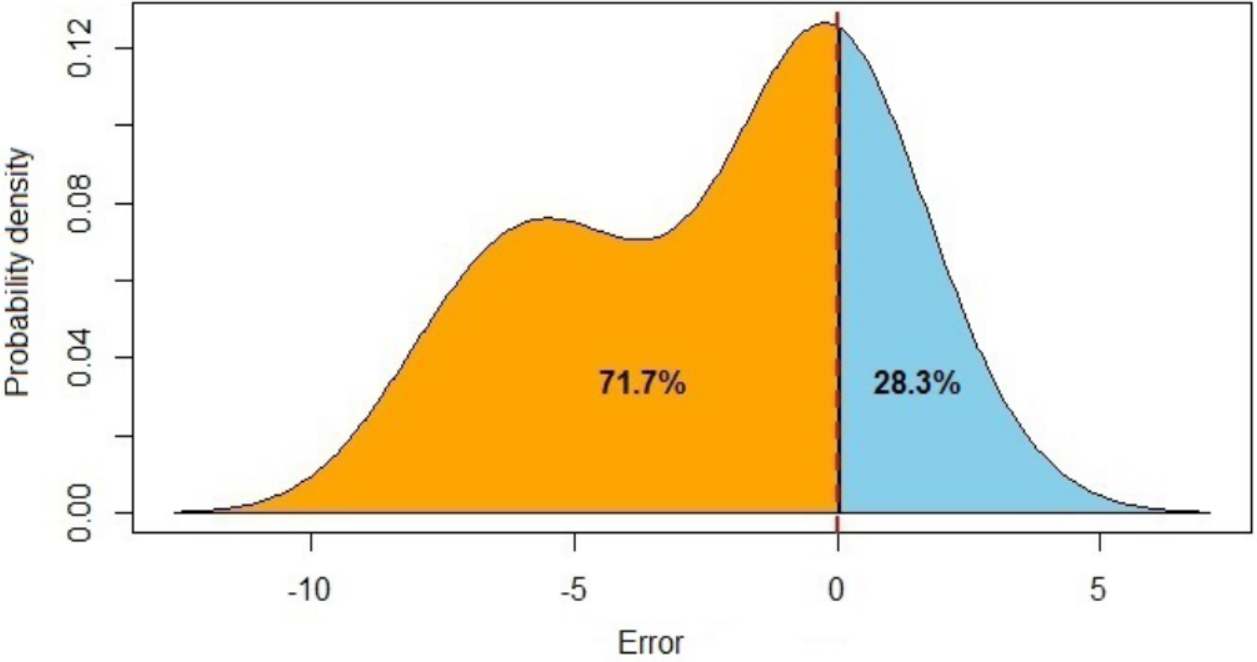
\includegraphics[width=0.8\linewidth]{images/figure6a.png}
  }\par        
\subfloat[\textbf{Evaluative type (Problem).}\label{fig:f6b}]{
  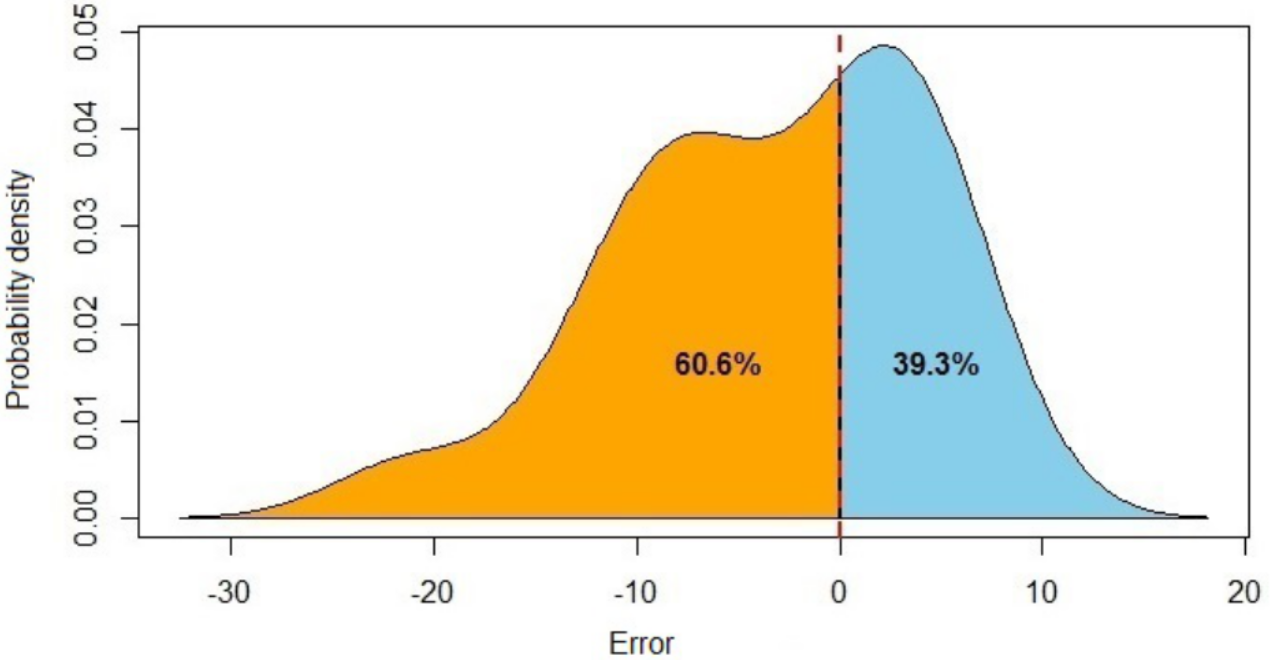
\includegraphics[width=0.8\linewidth]{images/figure6b.png}
  }
\caption{\textbf{Probability density of Error for estimating time for
different LO using Median method. Timescale is in minutes.}}
\label{fig:f6}
\end{minipage}
\end{figure}

\begin{figure}[t]
    \centering
    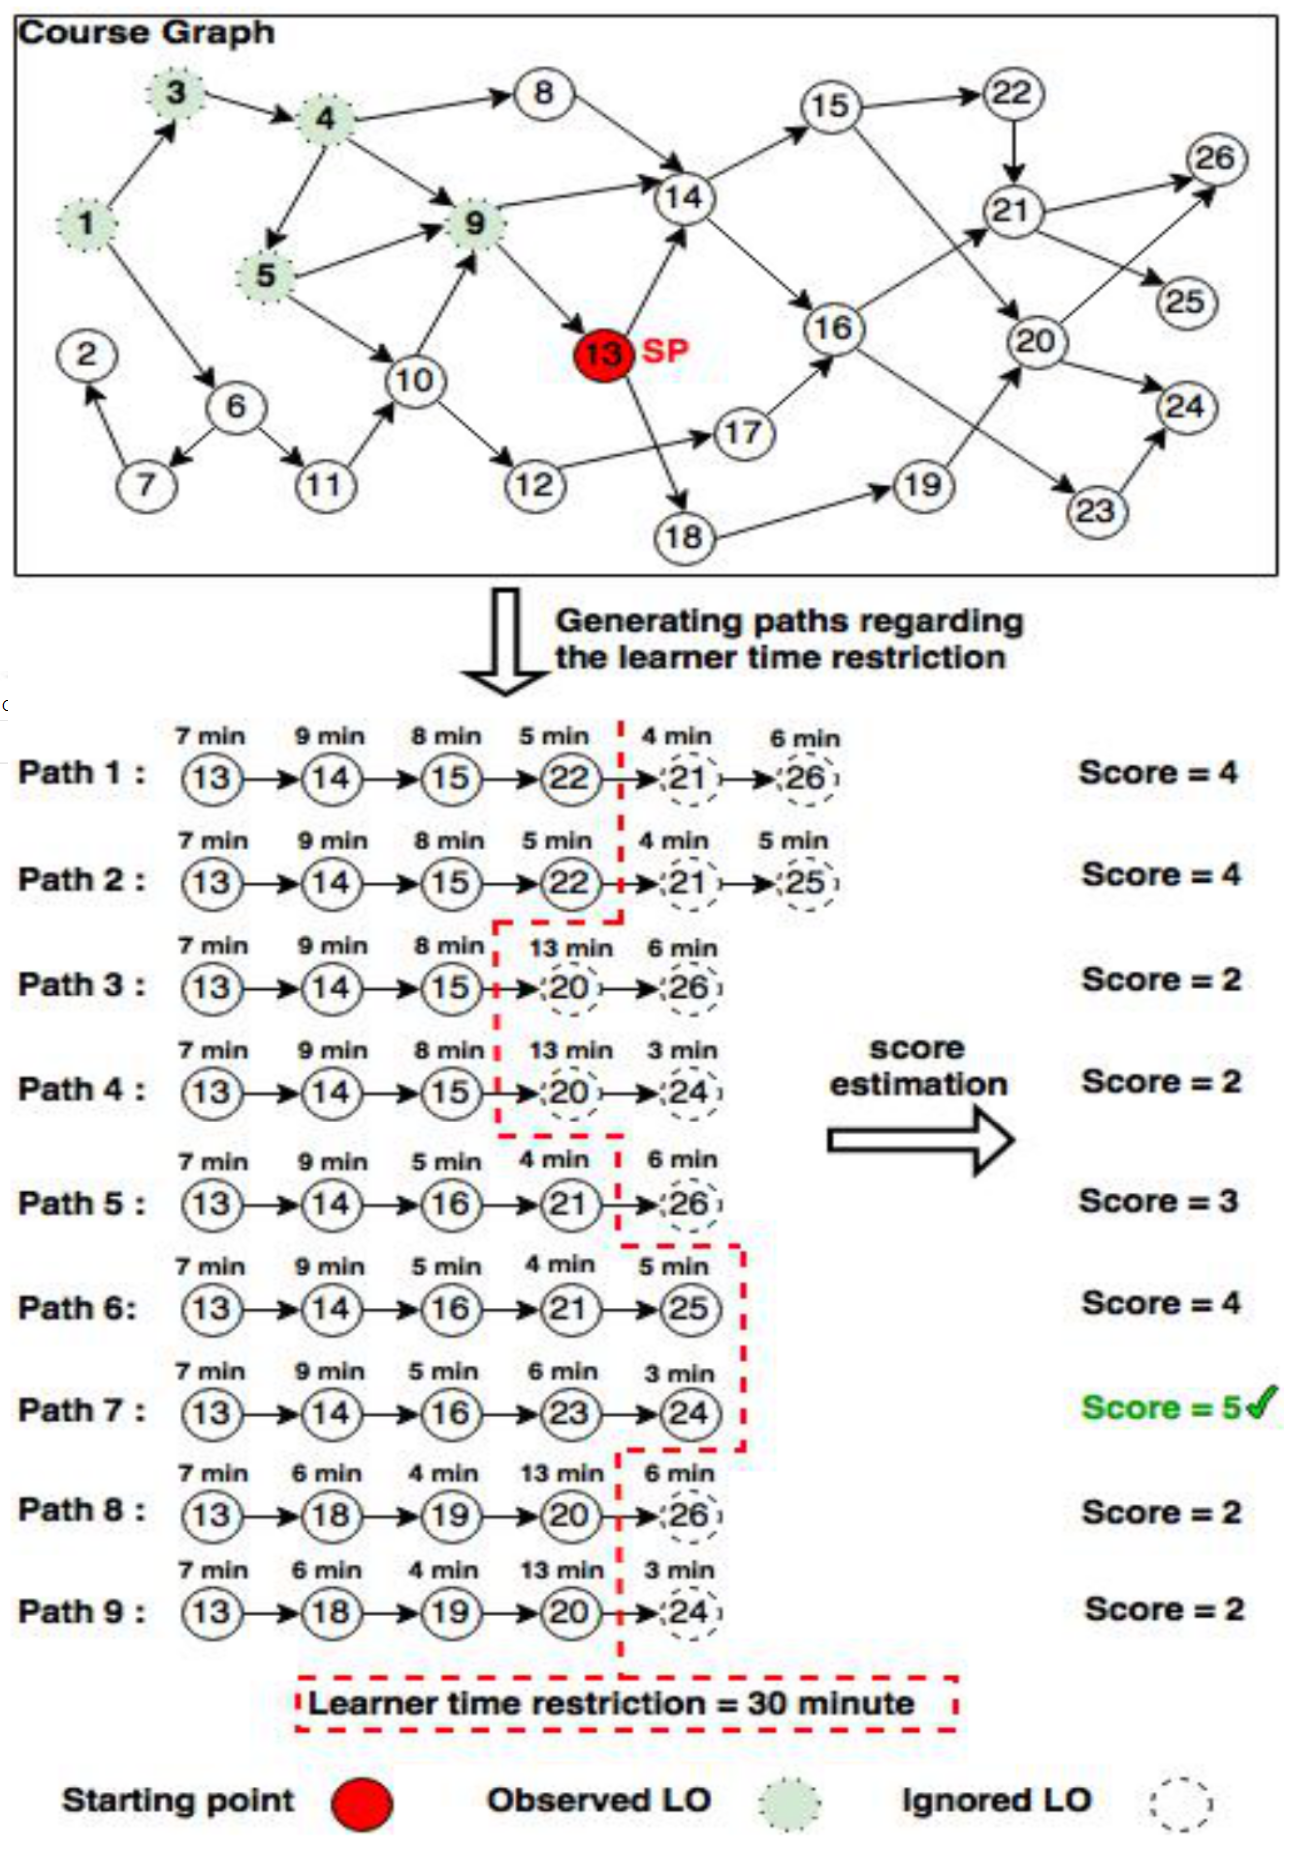
\includegraphics[width=0.8\linewidth]{images/figure7.png}
    \caption{\textbf{RUTICO example.}}
    \label{fig:f7}
\end{figure}

\noindent within project ”POCI-01-0145-FEDER-006961”, and by National Funds through the FCT - Fundação para a Ciência e a Tecnologia (Portuguese Foundation for Science and Technology) as part of project UID/EEA/50014/2013. The first author would like to thank José Carlos Paiva who was assisting during the data collection.

\bibliography{sample}
\balancecolumns
\end{document}